% SUTD-PRCM unit cell (dimensions in mm; layer thicknesses exaggerated for visibility).
% The copper pattern is a real layout (../data/layout_bits.tex, from data:architecture).
\documentclass[border=1pt]{standalone}
\usepackage[T1]{fontenc}\usepackage{helvet}\renewcommand{\familydefault}{\sfdefault}\usepackage{newtxsf}
\usepackage{tikz}
\usetikzlibrary{arrows.meta,calc}
\input{../data/layout_bits.tex}

\definecolor{ink}{HTML}{2B2B2B}
\definecolor{muted}{HTML}{6B6B6B}
\definecolor{bbC}{HTML}{3D74B8}
\definecolor{pgaC}{HTML}{E0704A}
\definecolor{cuTop}{HTML}{D9904A}
\definecolor{cuFront}{HTML}{A8662C}
\definecolor{cuSide}{HTML}{BF7838}
\definecolor{gnd}{HTML}{9C7B5B}
\definecolor{subTop}{HTML}{EFEADB}
\definecolor{subFront}{HTML}{D8D0B5}
\definecolor{subSide}{HTML}{E4DDC6}

\tikzset{
  >={Stealth[length=3.6pt,width=3.2pt]},
  lbl/.style={font=\fontsize{8}{9.4}\selectfont,text=ink,align=left,inner sep=1pt},
  sub/.style={font=\fontsize{8}{9.4}\selectfont,text=muted,align=left,inner sep=1pt},
  dim/.style={<->,line width=0.4pt,draw=muted,>={Stealth[length=2.6pt,width=2.4pt]}},
}

\begin{document}
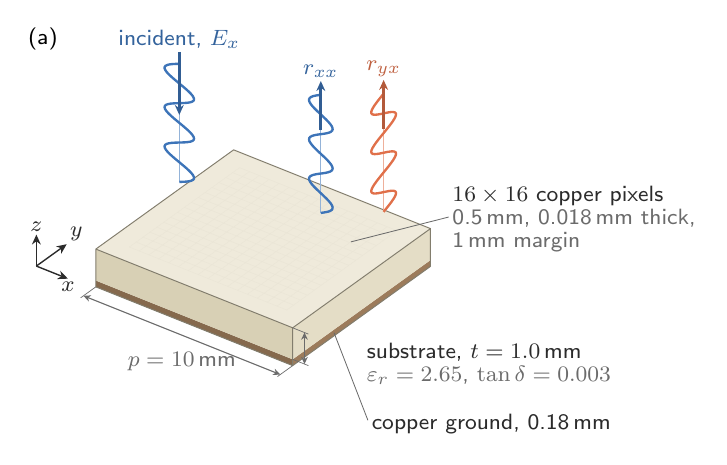
\begin{tikzpicture}[x={(0.25cm,-0.10cm)},y={(0.175cm,0.126cm)},z={(0cm,0.25cm)}]
\def\zt{1.6}\def\zc{1.82}\def\zg{-0.32}

% copper ground plane
\fill[gnd!85!black] (0,0,\zg) -- (10,0,\zg) -- (10,0,0) -- (0,0,0) -- cycle;
\fill[gnd] (10,0,\zg) -- (10,10,\zg) -- (10,10,0) -- (10,0,0) -- cycle;
% substrate
\fill[subFront] (0,0,0) -- (10,0,0) -- (10,0,\zt) -- (0,0,\zt) -- cycle;
\fill[subSide] (10,0,0) -- (10,10,0) -- (10,10,\zt) -- (10,0,\zt) -- cycle;
\fill[subTop] (0,0,\zt) -- (10,0,\zt) -- (10,10,\zt) -- (0,10,\zt) -- cycle;
\draw[subFront!60!black,line width=0.35pt] (0,0,\zg) -- (10,0,\zg) -- (10,10,\zg) (10,10,\zg) -- (10,10,\zt)
  -- (0,10,\zt) -- (0,0,\zt) -- (0,0,\zg) (0,0,\zt) -- (10,0,\zt) -- (10,10,\zt) (10,0,\zt) -- (10,0,\zg);
% pixel grid footprint (16 x 16, 0.5 mm, 1 mm margin)
\foreach \i in {0,...,16}{
  \draw[subFront!55,line width=0.15pt] (1+\i*0.5,1,\zt) -- (1+\i*0.5,9,\zt);
  \draw[subFront!55,line width=0.15pt] (1,1+\i*0.5,\zt) -- (9,1+\i*0.5,\zt);
}
% copper pixels, painted back (row 0) to front
\foreach \r/\c in \layoutbits{
  \pgfmathsetmacro{\xa}{1+0.5*\c}\pgfmathsetmacro{\xb}{\xa+0.5}
  \pgfmathsetmacro{\ya}{8.5-0.5*\r}\pgfmathsetmacro{\yb}{\ya+0.5}
  \fill[cuFront] (\xa,\ya,\zt) -- (\xb,\ya,\zt) -- (\xb,\ya,\zc) -- (\xa,\ya,\zc) -- cycle;
  \fill[cuSide] (\xb,\ya,\zt) -- (\xb,\yb,\zt) -- (\xb,\yb,\zc) -- (\xb,\ya,\zc) -- cycle;
  \fill[cuTop] (\xa,\ya,\zc) -- (\xb,\ya,\zc) -- (\xb,\yb,\zc) -- (\xa,\yb,\zc) -- cycle;
}

% incident x-polarised wave (E along x, travelling -z) and the two reflected components
\newcommand{\wave}[7]{% #1 x, #2 y, #3 z0, #4 z1, #5 colour, #6 ax (x amplitude), #7 ay (y amplitude)
  \draw[#5!55,line width=0.3pt] (#1,#2,#3) -- (#1,#2,#4);
  \draw[#5,line width=0.85pt,domain=#3:#4,samples=80,variable=\t]
    plot ({#1+#6*sin(deg(2*pi*(\t-#3)/2.0))},{#2+#7*sin(deg(2*pi*(\t-#3)/2.0))},{\t});}
\wave{2.0}{3.2}{4.2}{10.2}{bbC}{0.75}{0}
\draw[->,bbC!80!black,line width=1.0pt] (2.0,3.2,10.8) -- (2.0,3.2,7.6);
\node[lbl,text=bbC!85!black,anchor=south] at (2.0,3.2,10.8) {incident, $E_x$};
\wave{6.6}{6.9}{2.6}{8.6}{bbC}{0.6}{0}
\draw[->,bbC!80!black,line width=1.0pt] (6.6,6.9,6.8) -- (6.6,6.9,9.3);
\node[lbl,text=bbC!85!black,anchor=south] at (6.6,6.9,9.3) {$r_{xx}$};
\wave{8.6}{8.6}{2.6}{8.6}{pgaC}{0}{0.9}
\draw[->,pgaC!80!black,line width=1.0pt] (8.6,8.6,6.8) -- (8.6,8.6,9.3);
\node[lbl,text=pgaC!85!black,anchor=south] at (8.6,8.6,9.3) {$r_{yx}$};

% axes triad
\begin{scope}[shift={(-2.6,-0.6,0)}]
  \draw[->,ink,line width=0.5pt] (0,0,0) -- (1.6,0,0) node[lbl,anchor=north] {$x$};
  \draw[->,ink,line width=0.5pt] (0,0,0) -- (0,2.2,0) node[lbl,anchor=south west] {$y$};
  \draw[->,ink,line width=0.5pt] (0,0,0) -- (0,0,1.6) node[lbl,anchor=south] {$z$};
\end{scope}

% dimensions
\draw[dim] (0,-0.9,\zg) -- node[sub,anchor=north,yshift=-5pt] {$p=10$\,mm} (10,-0.9,\zg);
\draw[muted,line width=0.25pt] (0,0,\zg) -- (0,-1.1,\zg) (10,0,\zg) -- (10,-1.1,\zg);
\coordinate (tlab) at (10.9,0,\zt/2);
\draw[dim] (10.6,0,0) -- (10.6,0,\zt);
\draw[muted,line width=0.25pt] (10,0,0) -- (10.8,0,0) (10,0,\zt) -- (10.8,0,\zt);

% labels
\node[lbl,anchor=west] at (13.6,0,\zt/2+0.4) {substrate, $t=1.0$\,mm\\[-1pt]{\color{muted}$\varepsilon_r=2.65$, $\tan\delta=0.003$}};
\node[lbl,anchor=west] at (12.8,1.5,\zg-2.6) {copper ground, 0.18\,mm};
\draw[muted,line width=0.3pt] (10,3,\zg/2) -- (12.7,1.6,\zg-2.5);
\node[lbl,anchor=west] at (13.4,6.5,\zc+3.4) {$16\times16$ copper pixels\\[-1pt]{\color{muted}0.5\,mm, 0.018\,mm thick,}\\[-1pt]{\color{muted}1\,mm margin}};
\draw[muted,line width=0.3pt] (8.2,6.8,\zc) -- (13.3,6.6,\zc+3.4);

\node[anchor=north west,inner sep=0pt,font=\fontsize{8}{9}\selectfont] at (current bounding box.north west) {(a)};
\end{tikzpicture}
\end{document}
